%% Run LaTeX on this file several times to get Table of Contents,
%% cross-references, and citations.

\documentclass[11pt]{book}
\usepackage{array}
\usepackage{gvv}
\usepackage{gvv-book-bkup}
%\usepackage{Wiley-AuthoringTemplate}
\usepackage[sectionbib,authoryear]{natbib}% for name-date citation comment the below line
%\usepackage[sectionbib,numbers]{natbib}% for numbered citation comment the above line

%%********************************************************************%%
%%       How many levels of section head would you like numbered?     %%
%% 0= no section numbers, 1= section, 2= subsection, 3= subsubsection %%
\setcounter{secnumdepth}{3}
%%********************************************************************%%
%%**********************************************************************%%
%%     How many levels of section head would you like to appear in the  %%
%%				Table of Contents?			%%
%% 0= chapter, 1= section, 2= subsection, 3= subsubsection titles.	%%
\setcounter{tocdepth}{2}
%%**********************************************************************%%

%\includeonly{ch01}
\makeindex

\begin{document}

\frontmatter
%%%%%%%%%%%%%%%%%%%%%%%%%%%%%%%%%%%%%%%%%%%%%%%%%%%%%%%%%%%%%%%%
%% Title Pages
%% Wiley will provide title and copyright page, but you can make
%% your own titlepages if you'd like anyway
%% Setting up title pages, type in the appropriate names here:

\booktitle{CBSE Math}

\subtitle{Made Simple}

\AuAff{G. V. V. Sharma}


%% \\ will start a new line.
%% You may add \affil{} for affiliation, ie,
%\authors{Robert M. Groves\\
%\affil{Universitat de les Illes Balears}
%Floyd J. Fowler, Jr.\\
%\affil{University of New Mexico}
%}

%% Print Half Title and Title Page:
%\halftitlepage
\titlepage

%%%%%%%%%%%%%%%%%%%%%%%%%%%%%%%%%%%%%%%%%%%%%%%%%%%%%%%%%%%%%%%%
%% Copyright Page

\begin{copyrightpage}{2023}
%Title, etc
\end{copyrightpage}

% Note, you must use \ to start indented lines, ie,
% 
% \begin{copyrightpage}{2004}
% Survey Methodology / Robert M. Groves . . . [et al.].
% \       p. cm.---(Wiley series in survey methodology)
% \    ``Wiley-Interscience."
% \    Includes bibliographical references and index.
% \    ISBN 0-471-48348-6 (pbk.)
% \    1. Surveys---Methodology.  2. Social 
% \  sciences---Research---Statistical methods.  I. Groves, Robert M.  II. %
% Series.\\

% HA31.2.S873 2004
% 001.4'33---dc22                                             2004044064
% \end{copyrightpage}

%%%%%%%%%%%%%%%%%%%%%%%%%%%%%%%%%%%%%%%%%%%%%%%%%%%%%%%%%%%%%%%%
%% Only Dedication (optional) 

%\dedication{To my parents}

\tableofcontents

%\listoffigures %optional
%\listoftables  %optional

%% or Contributor Page for edited books
%% before \tableofcontents

%%%%%%%%%%%%%%%%%%%%%%%%%%%%%%%%%%%%%%%%%%%%%%%%%%%%%%%%%%%%%%%%
%  Contributors Page for Edited Book
%%%%%%%%%%%%%%%%%%%%%%%%%%%%%%%%%%%%%%%%%%%%%%%%%%%%%%%%%%%%%%%%

% If your book has chapters written by different authors,
% you'll need a Contributors page.

% Use \begin{contributors}...\end{contributors} and
% then enter each author with the \name{} command, followed
% by the affiliation information.

% \begin{contributors}
% \name{Masayki Abe,} Fujitsu Laboratories Ltd., Fujitsu Limited, Atsugi, Japan
%
% \name{L. A. Akers,} Center for Solid State Electronics Research, Arizona State University, Tempe, Arizona
%
% \name{G. H. Bernstein,} Department of Electrical and Computer Engineering, University of Notre Dame, Notre Dame, South Bend, Indiana; formerly of
% Center for Solid State Electronics Research, Arizona
% State University, Tempe, Arizona 
% \end{contributors}

%%%%%%%%%%%%%%%%%%%%%%%%%%%%%%%%%%%%%%%%%%%%%%%%%%%%%%%%%%%%%%%%
% Optional Foreword:

%\begin{foreword}
%\lipsum[1-2]
%\end{foreword}

%%%%%%%%%%%%%%%%%%%%%%%%%%%%%%%%%%%%%%%%%%%%%%%%%%%%%%%%%%%%%%%%
% Optional Preface:

%\begin{preface}
%\lipsum[1-1]
%\prefaceauthor{}
%\where{place\\
% date}
%\end{preface}

% ie,
% \begin{preface}
% This is an example preface.
% \prefaceauthor{R. K. Watts}
% \where{Durham, North Carolina\\
% September, 2004}

%%%%%%%%%%%%%%%%%%%%%%%%%%%%%%%%%%%%%%%%%%%%%%%%%%%%%%%%%%%%%%%%
% Optional Acknowledgments:

%\acknowledgments
%\lipsum[1-2]
%\authorinitials{I. R. S.}  

%%%%%%%%%%%%%%%%%%%%%%%%%%%%%%%%
%% Glossary Type of Environment:

% \begin{glossary}
% \term{<term>}{<description>}
% \end{glossary}

%%%%%%%%%%%%%%%%%%%%%%%%%%%%%%%%
%\begin{acronyms}
%\acro{ASTA}{Arrivals See Time Averages}
%\acro{BHCA}{Busy Hour Call Attempts}
%\acro{BR}{Bandwidth Reservation}
%\acro{b.u.}{bandwidth unit(s)}
%\acro{CAC}{Call / Connection Admission Control}
%\acro{CBP}{Call Blocking Probability(-ies)}
%\acro{CCS}{Centum Call Seconds}
%\acro{CDTM}{Connection Dependent Threshold Model}
%\acro{CS}{Complete Sharing}
%\acro{DiffServ}{Differentiated Services}
%\acro{EMLM}{Erlang Multirate Loss Model}
%\acro{erl}{The Erlang unit of traffic-load}
%\acro{FIFO}{First in - First out}
%\acro{GB}{Global balance}
%\acro{GoS}{Grade of Service}
%\acro{ICT}{Information and Communication Technology}
%\acro{IntServ}{Integrated Services}
%\acro{IP}{Internet Protocol}
%\acro{ITU-T}{International Telecommunication Unit -- Standardization sector}
%\acro{LB}{Local balance}
%\acro{LHS}{Left hand side}
%\acro{LIFO}{Last in - First out}
%\acro{MMPP}{Markov Modulated Poisson Process}
%\acro{MPLS}{Multiple Protocol Labeling Switching}
%\acro{MRM}{Multi-Retry Model}
%\acro{MTM}{Multi-Threshold Model}
%\acro{PASTA}{Poisson Arrivals See Time Averages}
%\acro{PDF}{Probability Distribution Function}
%\acro{pdf}{probability density function}
%\acro{PFS}{Product Form Solution}
%\acro{QoS}{Quality of Service}
%\acro{r.v.}{random variable(s)}
%\acro{RED}{random early detection}
%\acro{RHS}{Right hand side}
%\acro{RLA}{Reduced Load Approximation}
%\acro{SIRO}{service in random order}
%\acro{SRM}{Single-Retry Model}
%\acro{STM}{Single-Threshold Model}
%\acro{TCP}{Transport Control Protocol}
%\acro{TH}{Threshold(s)}
%\acro{UDP}{User Datagram Protocol}
%\end{acronyms}

\setcounter{page}{1}

\begin{introduction}
This book links high school coordinate geometry to linear algebra and matrix analysis through solved problems.

\end{introduction}

\mainmatter
\chapter{Intersection of Conics}
\section{Chords}
\begin{enumerate}[label=\thesection.\arabic*.,ref=\thesection.\theenumi]
\numberwithin{equation}{enumi}
\numberwithin{figure}{enumi}
\numberwithin{table}{enumi}
\item Using integration, find the area of the region enclosed by the curve $ y=x^2 $, the x-axis and the ordinates $x=-2$ \text { and } $x=1$.

\item Using integration, find the area of the region enclosed by line $y=\sqrt{3}x$ semi-circle $y=\sqrt{4-x^2}$ and x-axis in first quadrant.

\item Using integration, find the area of the smaller region enclosed by the curve ${4x^2 + 4y^2} = 9$ and the line $2x + 2y =3$.

\item If the area of the regin bounded by the curve $y^2 = 4ax$ and the line $x = 4a$ is $\dfrac{256}{3}$\hspace{0.2cm} sq. units, then using integration, find the value of a, where $a>0$.

\item Find the area of the region enclosed by the curves $y^2=x$, $x=\dfrac{1}{4}$,  $y=0$ and $x=1$, using integration.

\item If the area of the region bounded bythe line $y=mx$ and the curve $x^2=y$ is $\dfrac{32}{3}$\hspace{0.2cm}sq. units, then find the positive value of m, using integration.

\item If the area between the curves $x = y^2$ and $x = 4$ is divided into two equal parts by the line $x = a$, then find the value of a, using integration.

\item Find the area bounded by the ellipse $x^2+4y^2=16$ and the ordinates $x=0$ and $x=2$, using integration.

\item Find the area of the region $\{(x,y) : x^2 \leq y \leq x\}$, using integration

\end{enumerate}

\section{Curves}
\input{2022/curves.tex}
\chapter{Tangent And Normal}
\begin{enumerate}[label=\thesection.\arabic*.,ref=\thesection.\theenumi]
\numberwithin{equation}{enumi}
\numberwithin{figure}{enumi}
\numberwithin{table}{enumi}

	\item Draw a circle of radius 2.5 cm. Take a point $\vec{P}$ outside the circle at a distance of 7 cm from the center. Then construct a pair of tangents to the circle from point $\vec{P}$.

	\item Write the steps of construction for constructing a pair of tangents to a circle of radius 4 cm from a point $\vec{P}$, at a distance of 7 cm from its center $\vec{O}$.

	\item In Figure \ref{fig:tan1}, there are two concentric circles with centre $\vec{O}$. If $ARC$ and $AQB$ are tangents to the smaller circle  from the point $\vec{A}$ lying on the larger circle, find the length of $AC$, if $AQ$ = 5 cm.
		\begin{figure}[H]
			\centering
			
\includegraphics[width=\columnwidth]{figs/tan}
			\caption{Two concentric circles with $\vec{O}$ as centre}
			\label{fig:tan1}
		\end{figure}
	
	\item In Figure \ref{fig:cir1}, if a circle touches the side $QR$ of $\Delta PQR$ at $\vec{S}$ and extended sides $PQ$ and $PR$ at $\vec{M}$ and $\vec{N}$, respectively,
		\begin{figure}[H]
			\centering
			
\includegraphics[width=\columnwidth]{figs/cir}
				\caption{Two tangents are drawn from point $\vec{P}$ to the circle}
				\label{fig:cir1}
		\end{figure}
		prove that $PM=\dfrac{1}{2}(PQ+QR+PR)$

	\item In Figure \ref{fig:tri1}, a triangle $ABC$ is drawn to circumscribe a circle of radius 4 cm such that the segments $BD$ and $DC$ into which $BC$ is divided by the point of contact $\vec{D}$ are of lengths 6 cm and 8 cm respectively. If the area of $\Delta ABC$ is 84 $cm^2$, find the lengths of sides $AB$ and $AC$.
		\begin{figure}[H]
			\centering
			
\includegraphics[width=\columnwidth]{figs/tri}
				\caption{Circle with $\vec{O}$ as center circumscribed in triangle $ABC$}
				\label{fig:tri1}
		\end{figure}

	\item In Figure \ref{fig:sq1}, $PQ$ and $PR$ are tangents to the circle centered at $\vec{O}$. If $\angle OPR=45\degree$, then prove that $ORPQ$ is a square.
		\begin{figure}[H]
			\centering
			
\includegraphics[width=\columnwidth]{figs/sq}
			\caption{Two tangents drawn from point $\vec{P}$ to a circle whose centre is $\vec{O}$}
			\label{fig:sq1}
		\end{figure}

	\item In Figure \ref{fig:sct1}, $\vec{O}$ is the centre of a circle of radius 5 cm. $PA$ and $BC$ are tangents to the circle at $\vec{A}$ and $\vec{B}$ respectively. If $OP$ is 13 cm, then find the length of tangents $PA$ and $BC$.
		\begin{figure}[H]
			\centering
			
\includegraphics[width=\columnwidth]{figs/sct}
			\caption{Two tangents drawn from point $\vec{C}$ to a circle whose centre is $\vec{O}$}
			\label{fig:sct1}
		\end{figure}

	\item In Figure \ref{fig:ver1}, $AB$ is diameter of a circle centered at $\vec{O}$. $BC$ is tangent to the circle at $\vec{B}$. If $OP$ bisects the chord $AD$ and $\angle AOP=60\degree$, then find $m\angle C$.
		\begin{figure}[H]
			\centering
			
\includegraphics[width=\columnwidth]{figs/ver}
			\caption{Tangent $BC$ is drawn from point $\vec{C}$ to a circle whose centre is $\vec{O}$}
			\label{fig:ver1}
		\end{figure}

	\item In Figure \ref{fig:hor1}, $XAY$ is a tangent to the circle centered at $\vec{O}$. If $\angle ABO=60\degree$,then find $m\angle BAY$ and $m\angle AOB$.
		\begin{figure}
			\centering
			
\includegraphics[width=\columnwidth]{figs/hor}
			\caption{The line $XAY$ is tangent to the circle centered at $\vec{O}$}
			\label{fig:hor1}
		\end{figure}

	\item Two concentric circles are of radii 4cm and 3 cm. Find the length of the chord of the larger circle which touches the smaller circle.

	\item In Figure \ref{fig:sl1}, a triangle $ABC$ with $\angle B=90\degree$ is shown. Taking $AB$ as diameter, a circle has been drawn intersecting $AC$ at point $\vec{P}$. Prove that the tangent drawn at point $\vec{P}$ bisects $BC$.
		\begin{figure}[H]
			\centering
			
\includegraphics[width=\columnwidth]{figs/sl}
			\caption{$PQ$ is tangent to the circle centered at $\vec{O}$. $AB$ is the diameter and $\angle B=90\degree$}
			\label{fig:sl1}
		\end{figure}
\item Find the equation of tangent to the curve $y = x^2 + 4x + 1$ at the point $(3,22)$.
\end{enumerate}

\section{Construction}
\iffalse
\chapter{Vectors}
\section{Length}
\input{chapters/vectors/examples/length.tex}
\section{Distance}
\input{chapters/vectors/examples/distance.tex}
\section{Exercises}
\input{chapters/vectors/exer/distance.tex}
\section{Section Formula}
\input{chapters/vectors/examples/section.tex}
\section{Exercises}
\input{chapters/vectors/exer/section.tex}
\section{Rank}
\input{chapters/vectors/examples/rank.tex}
\section{Exercises}
\input{chapters/vectors/exer/rank.tex}
\section{Scalar Product}
\input{chapters/vectors/examples/scalar.tex}
\section{Exercises}
\input{chapters/vectors/exer/scalar.tex}
\section{Orthogonality}
\input{chapters/vectors/examples/ortho.tex}
\section{Exercises}
\input{chapters/vectors/exer/ortho.tex}
\section{Vector Product}
\input{chapters/vectors/examples/cross.tex}
\section{Exercises}
\input{chapters/vectors/exer/cross.tex}
\section{Miscellaneous}
%\documentclass{exam}
%\usepackage{float}
%\usepackage{array}
%\usepackage{enumitem}
%\usepackage{amsmath}
%\begin{document}
\begin{enumerate}
	
	\item Find the distance of the point $(1,-2,9)$ from the point of intersection of the line
		\begin{align}
			\vec{r}=4\hat{i}+2\hat{j}+7\hat{k}+\lambda(3\hat{i}+4\hat{j}+2\hat{k})
		\end{align}and the plane
		\begin{align}
			\vec{r}\cdot(\hat{i}-\hat{j}+\hat{k})=10.
		\end{align}

	\item Find the area bounded by the curves $y=\abs{x-1}$ and $y=1$, using integration.

	\item Find the coordinates of the point where the line through $(4,-3,-4)$ and $(3,-2,2)$ crosses the plane $2x+y+z=6$.

	\item Fit a straight line trend by the method of least squares and find the trend value for the year 2008 using the data from Table \ref{tab:LC}:
		\begin{table}[H]
			\caption{Table showing yearly trend of production of goods in lakh tonnes \label{tab:LC}}
			%%%%%%%%%%%%%%%%%%%%%%%%%%%%%%%%%%%%%%%%%%%%%%%%%%%%%%%%%%%%%%%%%%%%%%
%%                                                                  %%
%%  This is the header of a LaTeX2e file exported from Gnumeric.    %%
%%                                                                  %%
%%  This file can be compiled as it stands or included in another   %%
%%  LaTeX document. The table is based on the longtable package so  %%
%%  the longtable options (headers, footers...) can be set in the   %%
%%  preamble section below (see PRAMBLE).                           %%
%%                                                                  %%
%%  To include the file in another, the following two lines must be %%
%%  in the including file:                                          %%
%%        \def\inputGnumericTable{}                                 %%
%%  at the beginning of the file and:                               %%
%%        \input{name-of-this-file.tex}                             %%
%%  where the table is to be placed. Note also that the including   %%
%%  file must use the following packages for the table to be        %%
%%  rendered correctly:                                             %%
%%    \usepackage[latin1]{inputenc}                                 %%
%%    \usepackage{color}                                            %%
%%    \usepackage{array}                                            %%
%%    \usepackage{longtable}                                        %%
%%    \usepackage{calc}                                             %%
%%    \usepackage{multirow}                                         %%
%%    \usepackage{hhline}                                           %%
%%    \usepackage{ifthen}                                           %%
%%  optionally (for landscape tables embedded in another document): %%
%%    \usepackage{lscape}                                           %%
%%                                                                  %%
%%%%%%%%%%%%%%%%%%%%%%%%%%%%%%%%%%%%%%%%%%%%%%%%%%%%%%%%%%%%%%%%%%%%%%



%%  This section checks if we are begin input into another file or  %%
%%  the file will be compiled alone. First use a macro taken from   %%
%%  the TeXbook ex 7.7 (suggestion of Han-Wen Nienhuys).            %%
\def\ifundefined#1{\expandafter\ifx\csname#1\endcsname\relax}


%%  Check for the \def token for inputed files. If it is not        %%
%%  defined, the file will be processed as a standalone and the     %%
%%  preamble will be used.                                          %%
\ifundefined{inputGnumericTable}

%%  We must be able to close or not the document at the end.        %%
 \def\gnumericTableEnd{\end{document}}


%%%%%%%%%%%%%%%%%%%%%%%%%%%%%%%%%%%%%%%%%%%%%%%%%%%%%%%%%%%%%%%%%%%%%%
%%                                                                  %%
%%  This is the PREAMBLE. Change these values to get the right      %%
%%  paper size and other niceties.                                  %%
%%                                                                  %%
%%%%%%%%%%%%%%%%%%%%%%%%%%%%%%%%%%%%%%%%%%%%%%%%%%%%%%%%%%%%%%%%%%%%%%

 \documentclass[12pt%
     %,landscape%
                    ]{report}
       \usepackage[latin1]{inputenc}
       \usepackage{fullpage}
       \usepackage{color}
       \usepackage{array}
       \usepackage{longtable}
       \usepackage{calc}
       \usepackage{multirow}
       \usepackage{hhline}
       \usepackage{ifthen}

 \begin{document}


%%  End of the preamble for the standalone. The next section is for %%
%%  documents which are included into other LaTeX2e files.          %%
\else

%%  We are not a stand alone document. For a regular table, we will %%
%%  have no preamble and only define the closing to mean nothing.   %%
    \def\gnumericTableEnd{}

%%  If we want landscape mode in an embedded document, comment out  %%
%%  the line above and uncomment the two below. The table will      %%
%%  begin on a new page and run in landscape mode.                  %%
%       \def\gnumericTableEnd{\end{landscape}}
%       \begin{landscape}


%%  End of theelse clause for this file being \input.              %%
\fi

%%%%%%%%%%%%%%%%%%%%%%%%%%%%%%%%%%%%%%%%%%%%%%%%%%%%%%%%%%%%%%%%%%%%%%
%%                                                                  %%
%%  The rest is the gnumeric table, except for the closing          %%
%%  statement. Changes below will alter the table's appearance.     %%
%%                                                                  %%
%%%%%%%%%%%%%%%%%%%%%%%%%%%%%%%%%%%%%%%%%%%%%%%%%%%%%%%%%%%%%%%%%%%%%%

\providecommand{\gnumericmathit}[1]{#1} 
%%  Uncomment the next line if you would like your numbers to be in %%
%%  italics if they are italizised in the gnumeric table.           %%
%\renewcommand{\gnumericmathit}[1]{\mathit{#1}}
\providecommand{\gnumericPB}[1]%
{\let\gnumericTemp=\\#1\let\\=\gnumericTemp\hspace{0pt}}
 \ifundefined{gnumericTableWidthDefined}
        \newlength{\gnumericTableWidth}
        \newlength{\gnumericTableWidthComplete}
        \newlength{\gnumericMultiRowLength}
        \global\def\gnumericTableWidthDefined{}
 \fi
%% The following setting protects this code from babel shorthands.  %%
 \ifthenelse{\isundefined{\languageshorthands}}{}{\languageshorthands{english}}
%%  The default table format retains the relative column widths of  %%
%%  gnumeric. They can easily be changed to c, r or l. In that case %%
%%  you may want to comment out the next line and uncomment the one %%
%%  thereafter                                                      %%
\providecommand\gnumbox{\makebox[0pt]}
%%\providecommand\gnumbox[1][]{\makebox}

%% to adjust positions in multirow situations                       %%
\setlength{\bigstrutjot}{\jot}
\setlength{\extrarowheight}{\doublerulesep}

%%  The \setlongtables command keeps column widths the same across  %%
%%  pages. Simply comment out next line for varying column widths.  %%
\setlongtables

\setlength\gnumericTableWidth{%
 53pt+%
 53pt+%
 106pt+%
0pt}
\def\gumericNumCols{3}
\setlength\gnumericTableWidthComplete{\gnumericTableWidth+%
         \tabcolsep*\gumericNumCols*2+\arrayrulewidth*\gumericNumCols}
\ifthenelse{\lengthtest{\gnumericTableWidthComplete > \linewidth}}%
         {\def\gnumericScale{\ratio{\linewidth-%
                        \tabcolsep*\gumericNumCols*2-%
                        \arrayrulewidth*\gumericNumCols}%
{\gnumericTableWidth}}}%
{\def\gnumericScale{1}}

%%%%%%%%%%%%%%%%%%%%%%%%%%%%%%%%%%%%%%%%%%%%%%%%%%%%%%%%%%%%%%%%%%%%%%
%%                                                                  %%
%% The following are the widths of the various columns. We are      %%
%% defining them here because then they are easier to change.       %%
%% Depending on the cell formats we may use them more than once.    %%
%%                                                                  %%
%%%%%%%%%%%%%%%%%%%%%%%%%%%%%%%%%%%%%%%%%%%%%%%%%%%%%%%%%%%%%%%%%%%%%%

\ifthenelse{\isundefined{\gnumericColA}}{\newlength{\gnumericColA}}{}\settowidth{\gnumericColA}{\begin{tabular}{@{}p{53pt*\gnumericScale}@{}}x\end{tabular}}
\ifthenelse{\isundefined{\gnumericColB}}{\newlength{\gnumericColB}}{}\settowidth{\gnumericColB}{\begin{tabular}{@{}p{150pt*\gnumericScale}@{}}x\end{tabular}}
\ifthenelse{\isundefined{\gnumericColC}}{\newlength{\gnumericColC}}{}\settowidth{\gnumericColC}{\begin{tabular}{@{}p{106pt*\gnumericScale}@{}}x\end{tabular}}

\begin{longtable}[c]{%
 b{\gnumericColA}%
 b{\gnumericColB}%
 b{\gnumericColC}%
 }

%%%%%%%%%%%%%%%%%%%%%%%%%%%%%%%%%%%%%%%%%%%%%%%%%%%%%%%%%%%%%%%%%%%%%%
%%  The longtable options. (Caption, headers... see Goosens, p.124) %%
% \caption{The Table Caption.}             \\ %
% \hline % Across the top of the table.
%%  The rest of these options are table rows which are placed on    %%
%%  the first, last or every page. Use \multicolumn if you want.    %%

%%  Header for the first page.                                      %%
% \multicolumn{3}{c}{The First Header} \\ \hline 
% \multicolumn{1}{c}{colTag} %Column 1
% &\multicolumn{1}{c}{colTag} %Column 2
% &\multicolumn{1}{c}{colTag} \\ \hline %Last column
% \endfirsthead

%%  The running header deinition.

%%
% \hline
% \multicolumn{3}{l}{\ldots\small\slshape continued} \\ \hline
% \multicolumn{1}{c}{colTag} %Column 1
% &\multicolumn{1}{c}{colTag} %Column 2
% &\multicolumn{1}{c}{colTag} \\ \hline %Last column
% \endhead

%%  The running footer definition.                                  %%
% \hline
% \multicolumn{3}{r}{\small\slshape continued\ldots} \\
% \endfoot

%%  The ending footer definition.                                   %%
% \multicolumn{3}{c}{That's all folks} \\ \hline 
% \endlastfoot
%%%%%%%%%%%%%%%%%%%%%%%%%%%%%%%%%%%%%%%%%%%%%%%%%%%%%%%%%%%%%%%%%%%%%%

\hhline{|-|-|-}
  \multicolumn{1}{|p{\gnumericColA}|}%
 {\gnumericPB{\raggedright}\gnumbox[l]{Year}}
 &\multicolumn{1}{p{\gnumericColB}|}%
	{\gnumericPB{\raggedright}\gnumbox[l]{Production (in lakh tonnes)}}
 %&\multicolumn{1}{p{\gnumericColC}|}%
 %{\gnumericPB{\raggedright}\gnumbox[l]{Description}}
\\
\hhline{|---|}
  \multicolumn{1}{|p{\gnumericColA}|}%
 {\gnumericPB{\raggedright}\gnumbox[l]{2001}}
 &\multicolumn{1}{p{\gnumericColB}|}%
 {\gnumericPB{\raggedright}\gnumbox[l]{30}}
 %&\multicolumn{1}{p{\gnumericColC}|}%
 %{\gnumericPB{\raggedright}\gnumbox[l]{Vertex A}}
\\
\hhline{|---|}
  \multicolumn{1}{|p{\gnumericColA}|}%
 {\gnumericPB{\raggedright}\gnumbox[l]{2002}}
 &\multicolumn{1}{p{\gnumericColB}|}%
 {\gnumericPB{\raggedright}\gnumbox[l]{35}}
 %&\multicolumn{1}{p{\gnumericColC}|}%
 %{\gnumericPB{\raggedright}\gnumbox[l]{Vertex B}}
\\
\hhline{|---|}
  \multicolumn{1}{|p{\gnumericColA}|}%
 {\gnumericPB{\raggedright}\gnumbox[l]{2003}}
 &\multicolumn{1}{p{\gnumericColB}|}%
 {\gnumericPB{\raggedright}\gnumbox[l]{36}}
 %&\multicolumn{1}{p{\gnumericColC}|}%
 %{\gnumericPB{\raggedright}\gnumbox[l]{Vertex C}}
\\
\hhline{|---|}
  \multicolumn{1}{|p{\gnumericColA}|}%
 {\gnumericPB{\raggedright}\gnumbox[l]{2004}}
 &\multicolumn{1}{p{\gnumericColB}|}%
 {\gnumericPB{\raggedright}\gnumbox[l]{32}}
 %&\multicolumn{1}{p{\gnumericColC}|}%
 %{\gnumericPB{\raggedright}\gnumbox[l]{Midpoint of AC}}
\\
\hhline{|---|}
  \multicolumn{1}{|p{\gnumericColA}|}%
 {\gnumericPB{\raggedright}\gnumbox[l]{2005}}
 &\multicolumn{1}{p{\gnumericColB}|}%
 {\gnumericPB{\raggedright}\gnumbox[l]{37}}
 %&\multicolumn{1}{p{\gnumericColC}|}%
 %{\gnumericPB{\raggedright}\gnumbox[l]{Midpoint of BC}}
\\
\hhline{|---|}
  \multicolumn{1}{|p{\gnumericColA}|}%
 {\gnumericPB{\raggedright}\gnumbox[l]{2006}}
 &\multicolumn{1}{p{\gnumericColB}|}%
 {\gnumericPB{\raggedright}\gnumbox[l]{40}}
 %&\multicolumn{1}{p{\gnumericColC}|}%
 %{\gnumericPB{\raggedright}\gnumbox[l]{Midpoint of AB}}
\\
\hhline{|-|-|-|}
\end{longtable}

\ifthenelse{\isundefined{\languageshorthands}}{}{\languageshorthands{\languagename}}
\gnumericTableEnd

		\end{table}
\end{enumerate}
%\end{document}

\section{Exercises}
%\documentclass{exam}
%\usepackage{float}
%\usepackage{array}
%\usepackage{enumitem}
%\usepackage{amsmath}
%\begin{document}
\begin{enumerate}
	
	\item Find the distance of the point $(1,-2,9)$ from the point of intersection of the line
		\begin{align}
			\vec{r}=4\hat{i}+2\hat{j}+7\hat{k}+\lambda(3\hat{i}+4\hat{j}+2\hat{k})
		\end{align}and the plane
		\begin{align}
			\vec{r}\cdot(\hat{i}-\hat{j}+\hat{k})=10.
		\end{align}

	\item Find the area bounded by the curves $y=\abs{x-1}$ and $y=1$, using integration.

	\item Find the coordinates of the point where the line through $(4,-3,-4)$ and $(3,-2,2)$ crosses the plane $2x+y+z=6$.

	\item Fit a straight line trend by the method of least squares and find the trend value for the year 2008 using the data from Table \ref{tab:LC}:
		\begin{table}[H]
			\caption{Table showing yearly trend of production of goods in lakh tonnes \label{tab:LC}}
			%%%%%%%%%%%%%%%%%%%%%%%%%%%%%%%%%%%%%%%%%%%%%%%%%%%%%%%%%%%%%%%%%%%%%%
%%                                                                  %%
%%  This is the header of a LaTeX2e file exported from Gnumeric.    %%
%%                                                                  %%
%%  This file can be compiled as it stands or included in another   %%
%%  LaTeX document. The table is based on the longtable package so  %%
%%  the longtable options (headers, footers...) can be set in the   %%
%%  preamble section below (see PRAMBLE).                           %%
%%                                                                  %%
%%  To include the file in another, the following two lines must be %%
%%  in the including file:                                          %%
%%        \def\inputGnumericTable{}                                 %%
%%  at the beginning of the file and:                               %%
%%        \input{name-of-this-file.tex}                             %%
%%  where the table is to be placed. Note also that the including   %%
%%  file must use the following packages for the table to be        %%
%%  rendered correctly:                                             %%
%%    \usepackage[latin1]{inputenc}                                 %%
%%    \usepackage{color}                                            %%
%%    \usepackage{array}                                            %%
%%    \usepackage{longtable}                                        %%
%%    \usepackage{calc}                                             %%
%%    \usepackage{multirow}                                         %%
%%    \usepackage{hhline}                                           %%
%%    \usepackage{ifthen}                                           %%
%%  optionally (for landscape tables embedded in another document): %%
%%    \usepackage{lscape}                                           %%
%%                                                                  %%
%%%%%%%%%%%%%%%%%%%%%%%%%%%%%%%%%%%%%%%%%%%%%%%%%%%%%%%%%%%%%%%%%%%%%%



%%  This section checks if we are begin input into another file or  %%
%%  the file will be compiled alone. First use a macro taken from   %%
%%  the TeXbook ex 7.7 (suggestion of Han-Wen Nienhuys).            %%
\def\ifundefined#1{\expandafter\ifx\csname#1\endcsname\relax}


%%  Check for the \def token for inputed files. If it is not        %%
%%  defined, the file will be processed as a standalone and the     %%
%%  preamble will be used.                                          %%
\ifundefined{inputGnumericTable}

%%  We must be able to close or not the document at the end.        %%
 \def\gnumericTableEnd{\end{document}}


%%%%%%%%%%%%%%%%%%%%%%%%%%%%%%%%%%%%%%%%%%%%%%%%%%%%%%%%%%%%%%%%%%%%%%
%%                                                                  %%
%%  This is the PREAMBLE. Change these values to get the right      %%
%%  paper size and other niceties.                                  %%
%%                                                                  %%
%%%%%%%%%%%%%%%%%%%%%%%%%%%%%%%%%%%%%%%%%%%%%%%%%%%%%%%%%%%%%%%%%%%%%%

 \documentclass[12pt%
     %,landscape%
                    ]{report}
       \usepackage[latin1]{inputenc}
       \usepackage{fullpage}
       \usepackage{color}
       \usepackage{array}
       \usepackage{longtable}
       \usepackage{calc}
       \usepackage{multirow}
       \usepackage{hhline}
       \usepackage{ifthen}

 \begin{document}


%%  End of the preamble for the standalone. The next section is for %%
%%  documents which are included into other LaTeX2e files.          %%
\else

%%  We are not a stand alone document. For a regular table, we will %%
%%  have no preamble and only define the closing to mean nothing.   %%
    \def\gnumericTableEnd{}

%%  If we want landscape mode in an embedded document, comment out  %%
%%  the line above and uncomment the two below. The table will      %%
%%  begin on a new page and run in landscape mode.                  %%
%       \def\gnumericTableEnd{\end{landscape}}
%       \begin{landscape}


%%  End of theelse clause for this file being \input.              %%
\fi

%%%%%%%%%%%%%%%%%%%%%%%%%%%%%%%%%%%%%%%%%%%%%%%%%%%%%%%%%%%%%%%%%%%%%%
%%                                                                  %%
%%  The rest is the gnumeric table, except for the closing          %%
%%  statement. Changes below will alter the table's appearance.     %%
%%                                                                  %%
%%%%%%%%%%%%%%%%%%%%%%%%%%%%%%%%%%%%%%%%%%%%%%%%%%%%%%%%%%%%%%%%%%%%%%

\providecommand{\gnumericmathit}[1]{#1} 
%%  Uncomment the next line if you would like your numbers to be in %%
%%  italics if they are italizised in the gnumeric table.           %%
%\renewcommand{\gnumericmathit}[1]{\mathit{#1}}
\providecommand{\gnumericPB}[1]%
{\let\gnumericTemp=\\#1\let\\=\gnumericTemp\hspace{0pt}}
 \ifundefined{gnumericTableWidthDefined}
        \newlength{\gnumericTableWidth}
        \newlength{\gnumericTableWidthComplete}
        \newlength{\gnumericMultiRowLength}
        \global\def\gnumericTableWidthDefined{}
 \fi
%% The following setting protects this code from babel shorthands.  %%
 \ifthenelse{\isundefined{\languageshorthands}}{}{\languageshorthands{english}}
%%  The default table format retains the relative column widths of  %%
%%  gnumeric. They can easily be changed to c, r or l. In that case %%
%%  you may want to comment out the next line and uncomment the one %%
%%  thereafter                                                      %%
\providecommand\gnumbox{\makebox[0pt]}
%%\providecommand\gnumbox[1][]{\makebox}

%% to adjust positions in multirow situations                       %%
\setlength{\bigstrutjot}{\jot}
\setlength{\extrarowheight}{\doublerulesep}

%%  The \setlongtables command keeps column widths the same across  %%
%%  pages. Simply comment out next line for varying column widths.  %%
\setlongtables

\setlength\gnumericTableWidth{%
 53pt+%
 53pt+%
 106pt+%
0pt}
\def\gumericNumCols{3}
\setlength\gnumericTableWidthComplete{\gnumericTableWidth+%
         \tabcolsep*\gumericNumCols*2+\arrayrulewidth*\gumericNumCols}
\ifthenelse{\lengthtest{\gnumericTableWidthComplete > \linewidth}}%
         {\def\gnumericScale{\ratio{\linewidth-%
                        \tabcolsep*\gumericNumCols*2-%
                        \arrayrulewidth*\gumericNumCols}%
{\gnumericTableWidth}}}%
{\def\gnumericScale{1}}

%%%%%%%%%%%%%%%%%%%%%%%%%%%%%%%%%%%%%%%%%%%%%%%%%%%%%%%%%%%%%%%%%%%%%%
%%                                                                  %%
%% The following are the widths of the various columns. We are      %%
%% defining them here because then they are easier to change.       %%
%% Depending on the cell formats we may use them more than once.    %%
%%                                                                  %%
%%%%%%%%%%%%%%%%%%%%%%%%%%%%%%%%%%%%%%%%%%%%%%%%%%%%%%%%%%%%%%%%%%%%%%

\ifthenelse{\isundefined{\gnumericColA}}{\newlength{\gnumericColA}}{}\settowidth{\gnumericColA}{\begin{tabular}{@{}p{53pt*\gnumericScale}@{}}x\end{tabular}}
\ifthenelse{\isundefined{\gnumericColB}}{\newlength{\gnumericColB}}{}\settowidth{\gnumericColB}{\begin{tabular}{@{}p{150pt*\gnumericScale}@{}}x\end{tabular}}
\ifthenelse{\isundefined{\gnumericColC}}{\newlength{\gnumericColC}}{}\settowidth{\gnumericColC}{\begin{tabular}{@{}p{106pt*\gnumericScale}@{}}x\end{tabular}}

\begin{longtable}[c]{%
 b{\gnumericColA}%
 b{\gnumericColB}%
 b{\gnumericColC}%
 }

%%%%%%%%%%%%%%%%%%%%%%%%%%%%%%%%%%%%%%%%%%%%%%%%%%%%%%%%%%%%%%%%%%%%%%
%%  The longtable options. (Caption, headers... see Goosens, p.124) %%
% \caption{The Table Caption.}             \\ %
% \hline % Across the top of the table.
%%  The rest of these options are table rows which are placed on    %%
%%  the first, last or every page. Use \multicolumn if you want.    %%

%%  Header for the first page.                                      %%
% \multicolumn{3}{c}{The First Header} \\ \hline 
% \multicolumn{1}{c}{colTag} %Column 1
% &\multicolumn{1}{c}{colTag} %Column 2
% &\multicolumn{1}{c}{colTag} \\ \hline %Last column
% \endfirsthead

%%  The running header deinition.

%%
% \hline
% \multicolumn{3}{l}{\ldots\small\slshape continued} \\ \hline
% \multicolumn{1}{c}{colTag} %Column 1
% &\multicolumn{1}{c}{colTag} %Column 2
% &\multicolumn{1}{c}{colTag} \\ \hline %Last column
% \endhead

%%  The running footer definition.                                  %%
% \hline
% \multicolumn{3}{r}{\small\slshape continued\ldots} \\
% \endfoot

%%  The ending footer definition.                                   %%
% \multicolumn{3}{c}{That's all folks} \\ \hline 
% \endlastfoot
%%%%%%%%%%%%%%%%%%%%%%%%%%%%%%%%%%%%%%%%%%%%%%%%%%%%%%%%%%%%%%%%%%%%%%

\hhline{|-|-|-}
  \multicolumn{1}{|p{\gnumericColA}|}%
 {\gnumericPB{\raggedright}\gnumbox[l]{Year}}
 &\multicolumn{1}{p{\gnumericColB}|}%
	{\gnumericPB{\raggedright}\gnumbox[l]{Production (in lakh tonnes)}}
 %&\multicolumn{1}{p{\gnumericColC}|}%
 %{\gnumericPB{\raggedright}\gnumbox[l]{Description}}
\\
\hhline{|---|}
  \multicolumn{1}{|p{\gnumericColA}|}%
 {\gnumericPB{\raggedright}\gnumbox[l]{2001}}
 &\multicolumn{1}{p{\gnumericColB}|}%
 {\gnumericPB{\raggedright}\gnumbox[l]{30}}
 %&\multicolumn{1}{p{\gnumericColC}|}%
 %{\gnumericPB{\raggedright}\gnumbox[l]{Vertex A}}
\\
\hhline{|---|}
  \multicolumn{1}{|p{\gnumericColA}|}%
 {\gnumericPB{\raggedright}\gnumbox[l]{2002}}
 &\multicolumn{1}{p{\gnumericColB}|}%
 {\gnumericPB{\raggedright}\gnumbox[l]{35}}
 %&\multicolumn{1}{p{\gnumericColC}|}%
 %{\gnumericPB{\raggedright}\gnumbox[l]{Vertex B}}
\\
\hhline{|---|}
  \multicolumn{1}{|p{\gnumericColA}|}%
 {\gnumericPB{\raggedright}\gnumbox[l]{2003}}
 &\multicolumn{1}{p{\gnumericColB}|}%
 {\gnumericPB{\raggedright}\gnumbox[l]{36}}
 %&\multicolumn{1}{p{\gnumericColC}|}%
 %{\gnumericPB{\raggedright}\gnumbox[l]{Vertex C}}
\\
\hhline{|---|}
  \multicolumn{1}{|p{\gnumericColA}|}%
 {\gnumericPB{\raggedright}\gnumbox[l]{2004}}
 &\multicolumn{1}{p{\gnumericColB}|}%
 {\gnumericPB{\raggedright}\gnumbox[l]{32}}
 %&\multicolumn{1}{p{\gnumericColC}|}%
 %{\gnumericPB{\raggedright}\gnumbox[l]{Midpoint of AC}}
\\
\hhline{|---|}
  \multicolumn{1}{|p{\gnumericColA}|}%
 {\gnumericPB{\raggedright}\gnumbox[l]{2005}}
 &\multicolumn{1}{p{\gnumericColB}|}%
 {\gnumericPB{\raggedright}\gnumbox[l]{37}}
 %&\multicolumn{1}{p{\gnumericColC}|}%
 %{\gnumericPB{\raggedright}\gnumbox[l]{Midpoint of BC}}
\\
\hhline{|---|}
  \multicolumn{1}{|p{\gnumericColA}|}%
 {\gnumericPB{\raggedright}\gnumbox[l]{2006}}
 &\multicolumn{1}{p{\gnumericColB}|}%
 {\gnumericPB{\raggedright}\gnumbox[l]{40}}
 %&\multicolumn{1}{p{\gnumericColC}|}%
 %{\gnumericPB{\raggedright}\gnumbox[l]{Midpoint of AB}}
\\
\hhline{|-|-|-|}
\end{longtable}

\ifthenelse{\isundefined{\languageshorthands}}{}{\languageshorthands{\languagename}}
\gnumericTableEnd

		\end{table}
\end{enumerate}
%\end{document}

\section{Triangle}
\input{chapters/const/examples/tri.tex}
\section{Exercises}
\input{chapters/const/exer/tri.tex}
\section{ Quadrilateral}
\input{chapters/const/examples/quad.tex}
\section{Exercises}
\input{chapters/const/exer/quad.tex}
\else
\chapter{Linear Forms}
\section{Equation of a Line}
%\documentclass{exam}
%\usepackage{enumitem}
%\usepackage{array}
%\usepackage{amsmath}
%\usepackage{float}
%\usepackage{graphicx}
%\begin{document}
\begin{enumerate}

	\item Solve the equations $x+2y=6$ and $2x-5y=12$ graphically.	

	\item Solve the following equations for $x$ and $y$ using cross-multiplication method:
		\begin{align}
			(ax-by)+(a+4b)=0\\(bx+ay)+(b-4a)=0
		\end{align}

	\item Find the co-ordinates of the point where the line $\dfrac{x-3}{-1}=\dfrac{y+4}{1}=\dfrac{z+5}{6}$ crosses the plane passing through the points $\left(\dfrac{7}{2},0,0\right),(0,7,0),(0,0,7)$.

	\item Electrical transmission wires which are laid down in winters are stretched tightly to accommodate expansion in summers.
		\begin{figure}[H]
			\centering
			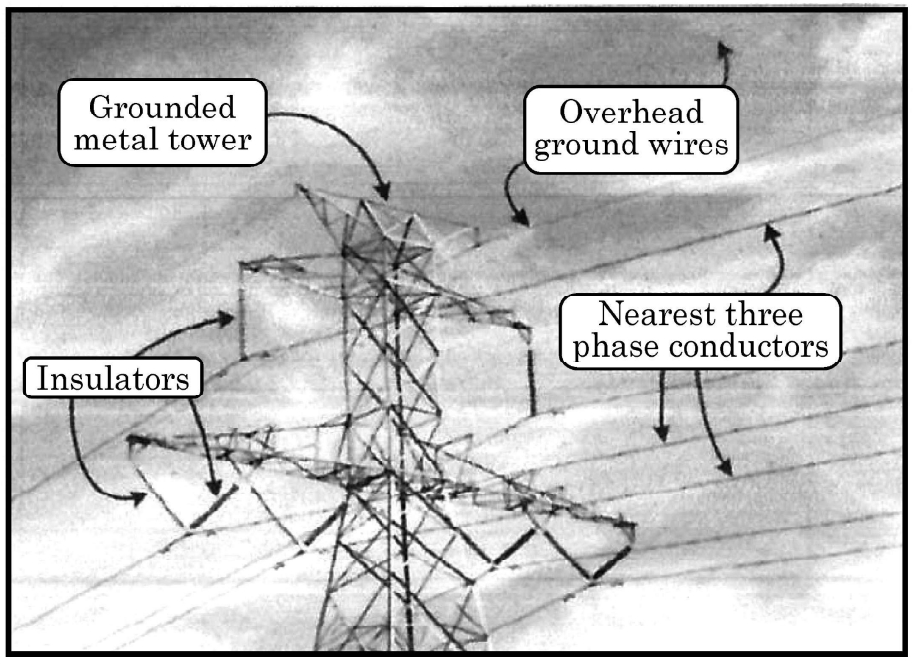
\includegraphics[width=\columnwidth]{figs/txn}
			\caption{Electrical transmission wires connected to a transmission tower.}
			\label{fig:txn1}
		\end{figure}
		Two such wires in the figure \ref{fig:txn1} lie along the following lines:
		\begin{align}
			l_1 &: \dfrac{x+1}{3}=\dfrac{y-3}{-2}=\dfrac{z+2}{-1}\\
			l_2 &: \dfrac{x}{-1}=\dfrac{y-7}{3}=\dfrac{z+7}{-2}
		\end{align}
		Based on the given information, answer the following questions:
		\begin{enumerate}
			\item	Are the $l_1$ and $l_2$ coplanar? Justify your answer.
			\item    Find the point of intersection of lines $l_1$ and $l_2$.
		\end{enumerate}

	\item Write the cartesian equation of the line PQ passing through points P$(2,2,1)$ and Q$(5,1,-2)$. Hence, find the y-coordinate of the point on the line PQ whose z-coordinate is -2.

	\item Find the distance between the lines $x=\dfrac{y-1}{2}=\dfrac{z-2}{3}$ and $x+1=\dfrac{y+2}{2}=\dfrac{z-1}{3}$.
	
	\item Find the shortest distance between the following lines:
		\begin{align}
			\vec{r}&=3\hat{i}+5\hat{j}+7\hat{k}+\lambda(\hat{i}-2\hat{j}+\hat{k})\\\vec{r}&=(-\hat{i}-\hat{j}-\hat{k})+\mu(7\hat{i}-6\hat{j}+\hat{k})
		\end{align}

	\item Two motorcycles A and B are running at a speed more than the allowed speed on the road (as shown in figure \ref{fig:bike1}) represented by the following lines 
		\begin{align}
			\vec{r}&=\lambda(\hat{i}+2\hat{j}-\hat{k})\\\vec{r}&=(3\hat{i}+3\hat{j})+\mu(2\hat{i}+\hat{j}+\hat{k})
		\end{align}
		\begin{figure}[H]
			\centering
			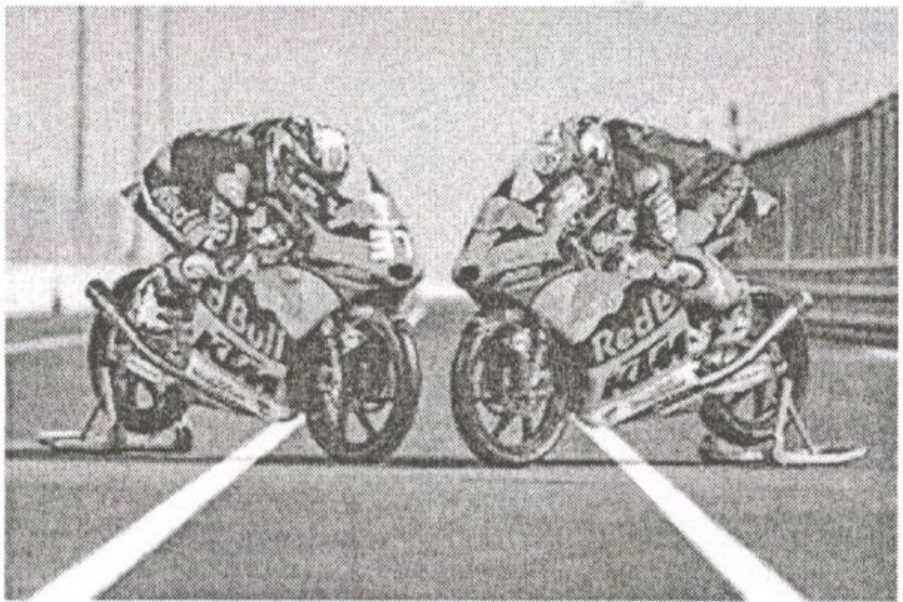
\includegraphics[width=\columnwidth]{figs/bike}
			\caption{Two motorcycles moving along the road in a straight line.}
			\label{fig:bike1}
		\end{figure}
		Based on the following information, answer the following questions:
		\begin{enumerate}
			\item Find the shortest distance between the given lines.
			\item Find a point at which the motorcycles may collide.
		\end{enumerate}
	
	\item Find the shortest distance between the following lines
		\begin{align}
			\vec{r}&=(\lambda+1)\hat{i}+(\lambda+4)\hat{j}-(\lambda-3)\hat{k}\\\vec{r}&=(3-\mu)\hat{i}+(2\mu+2)\hat{j}+(\mu+6)\hat{k}
		\end{align}
	
	\item Find the shortest distance between the following lines and hence write whether the lines are intersecting or not.
		\begin{align}
			\dfrac{x-1}{2}=\dfrac{y+1}{3}=z, \dfrac{x+1}{5}=\dfrac{y-2}{1}, z=2
		\end{align}
\end{enumerate}
%\end{document}

\section{Perpendicular}
%\documentclass{exam}
%\usepackage{amsmath}
%\usepackage{enumitem}
%\begin{document}
\begin{enumerate}

	\item If the distance of the point $(1,1,1)$ from the plane $x-y+z+\lambda=0$ is $\dfrac{5}{\sqrt{3}}$, find the value(s) of $\lambda$.

	\item Find the distance of the point $(2,3,4)$ measured along the line $\dfrac{x-4}{3}=\dfrac{y+5}{6}=\dfrac{z+1}{2}$ from the plane $3x+2y+2z+5=0$.

	\item Find the distance of the point $P(4,3,2)$ from the plane determined by the points $A(-1,6,-5),B(-5,-2,3)$ and $C(2,4,-5)$.

	\item The distance of the line
		\begin{align}
		\vec{r}=(\hat{i}-\hat{j})+\lambda(\hat{i}+5\hat{j}+\hat{k})\end{align}
		from the plane
		\begin{align}
		\vec{r}\cdot(\hat{i}-\hat{j}+4\hat{k})=5\end{align}
		is
		\begin{enumerate}
			\item $\sqrt{2}$
			\item $\dfrac{1}{\sqrt{2}}$
			\item $\dfrac{1}{3\sqrt{2}}$
			\item $\dfrac{-2}{3\sqrt{2}}$
		\end{enumerate}

	\item Find a unit vector perpendicular to each of the vectors $(\vec{a}+\vec{b})$ and $(\vec{a}-\vec{b})$ where 
	\begin{align}
		\vec{a}&=\hat{i}+\hat{j}+\hat{k}\\\vec{b}&=\hat{i}+2\hat{j}+3\hat{k}
	\end{align}
\end{enumerate}
%\end{document}


\section{Plane}
%\documentclass{exam}
%\usepackage{enumitem}
%\usepackage{amsmath}
%\begin{document}
\begin{enumerate}

	\item Find the equation of the plane passing through the points $(2,1,0),(3,-2,-2)$ and $(1,1,7)$. Also, obtain its distance from the origin.

	\item The foot of a perpendicular drawn from the point $(-2,-1,-3)$ on a plane is $(1,-3,3)$. Find the equation of the plane.

	\item Find the cartesian and the vector equation of a plane which passes through the point $(3,2,0)$ and contains the line $\dfrac{x-3}{1}=\dfrac{y-6}{5}=\dfrac{z-4}{4}$.

	\item The distance between the planes $4x-4y+2z+5=0$ and $2x-2y+z+6=0$ is

		\begin{enumerate}

			\item $\dfrac{1}{6}$
			\item $\dfrac{7}{6}$
			\item $\dfrac{11}{6}$
			\item $\dfrac{16}{6}$
		\end{enumerate}

	\item Find the equation of the plane through the line of intersection of the planes
		\begin{align}
			\vec{r}\cdot(\hat{i}+3\hat{j})+6&=0\\\vec{r}\cdot(3\hat{i}-\hat{j}-4\hat{k})&=0
		\end{align}which is at a  unit distance from the origin.
\end{enumerate}
%\end{document}

\section{Miscellaneous }
%\documentclass{exam}
%\usepackage{float}
%\usepackage{array}
%\usepackage{enumitem}
%\usepackage{amsmath}
%\begin{document}
\begin{enumerate}
	
	\item Find the distance of the point $(1,-2,9)$ from the point of intersection of the line
		\begin{align}
			\vec{r}=4\hat{i}+2\hat{j}+7\hat{k}+\lambda(3\hat{i}+4\hat{j}+2\hat{k})
		\end{align}and the plane
		\begin{align}
			\vec{r}\cdot(\hat{i}-\hat{j}+\hat{k})=10.
		\end{align}

	\item Find the area bounded by the curves $y=\abs{x-1}$ and $y=1$, using integration.

	\item Find the coordinates of the point where the line through $(4,-3,-4)$ and $(3,-2,2)$ crosses the plane $2x+y+z=6$.

	\item Fit a straight line trend by the method of least squares and find the trend value for the year 2008 using the data from Table \ref{tab:LC}:
		\begin{table}[H]
			\caption{Table showing yearly trend of production of goods in lakh tonnes \label{tab:LC}}
			%%%%%%%%%%%%%%%%%%%%%%%%%%%%%%%%%%%%%%%%%%%%%%%%%%%%%%%%%%%%%%%%%%%%%%
%%                                                                  %%
%%  This is the header of a LaTeX2e file exported from Gnumeric.    %%
%%                                                                  %%
%%  This file can be compiled as it stands or included in another   %%
%%  LaTeX document. The table is based on the longtable package so  %%
%%  the longtable options (headers, footers...) can be set in the   %%
%%  preamble section below (see PRAMBLE).                           %%
%%                                                                  %%
%%  To include the file in another, the following two lines must be %%
%%  in the including file:                                          %%
%%        \def\inputGnumericTable{}                                 %%
%%  at the beginning of the file and:                               %%
%%        \input{name-of-this-file.tex}                             %%
%%  where the table is to be placed. Note also that the including   %%
%%  file must use the following packages for the table to be        %%
%%  rendered correctly:                                             %%
%%    \usepackage[latin1]{inputenc}                                 %%
%%    \usepackage{color}                                            %%
%%    \usepackage{array}                                            %%
%%    \usepackage{longtable}                                        %%
%%    \usepackage{calc}                                             %%
%%    \usepackage{multirow}                                         %%
%%    \usepackage{hhline}                                           %%
%%    \usepackage{ifthen}                                           %%
%%  optionally (for landscape tables embedded in another document): %%
%%    \usepackage{lscape}                                           %%
%%                                                                  %%
%%%%%%%%%%%%%%%%%%%%%%%%%%%%%%%%%%%%%%%%%%%%%%%%%%%%%%%%%%%%%%%%%%%%%%



%%  This section checks if we are begin input into another file or  %%
%%  the file will be compiled alone. First use a macro taken from   %%
%%  the TeXbook ex 7.7 (suggestion of Han-Wen Nienhuys).            %%
\def\ifundefined#1{\expandafter\ifx\csname#1\endcsname\relax}


%%  Check for the \def token for inputed files. If it is not        %%
%%  defined, the file will be processed as a standalone and the     %%
%%  preamble will be used.                                          %%
\ifundefined{inputGnumericTable}

%%  We must be able to close or not the document at the end.        %%
 \def\gnumericTableEnd{\end{document}}


%%%%%%%%%%%%%%%%%%%%%%%%%%%%%%%%%%%%%%%%%%%%%%%%%%%%%%%%%%%%%%%%%%%%%%
%%                                                                  %%
%%  This is the PREAMBLE. Change these values to get the right      %%
%%  paper size and other niceties.                                  %%
%%                                                                  %%
%%%%%%%%%%%%%%%%%%%%%%%%%%%%%%%%%%%%%%%%%%%%%%%%%%%%%%%%%%%%%%%%%%%%%%

 \documentclass[12pt%
     %,landscape%
                    ]{report}
       \usepackage[latin1]{inputenc}
       \usepackage{fullpage}
       \usepackage{color}
       \usepackage{array}
       \usepackage{longtable}
       \usepackage{calc}
       \usepackage{multirow}
       \usepackage{hhline}
       \usepackage{ifthen}

 \begin{document}


%%  End of the preamble for the standalone. The next section is for %%
%%  documents which are included into other LaTeX2e files.          %%
\else

%%  We are not a stand alone document. For a regular table, we will %%
%%  have no preamble and only define the closing to mean nothing.   %%
    \def\gnumericTableEnd{}

%%  If we want landscape mode in an embedded document, comment out  %%
%%  the line above and uncomment the two below. The table will      %%
%%  begin on a new page and run in landscape mode.                  %%
%       \def\gnumericTableEnd{\end{landscape}}
%       \begin{landscape}


%%  End of theelse clause for this file being \input.              %%
\fi

%%%%%%%%%%%%%%%%%%%%%%%%%%%%%%%%%%%%%%%%%%%%%%%%%%%%%%%%%%%%%%%%%%%%%%
%%                                                                  %%
%%  The rest is the gnumeric table, except for the closing          %%
%%  statement. Changes below will alter the table's appearance.     %%
%%                                                                  %%
%%%%%%%%%%%%%%%%%%%%%%%%%%%%%%%%%%%%%%%%%%%%%%%%%%%%%%%%%%%%%%%%%%%%%%

\providecommand{\gnumericmathit}[1]{#1} 
%%  Uncomment the next line if you would like your numbers to be in %%
%%  italics if they are italizised in the gnumeric table.           %%
%\renewcommand{\gnumericmathit}[1]{\mathit{#1}}
\providecommand{\gnumericPB}[1]%
{\let\gnumericTemp=\\#1\let\\=\gnumericTemp\hspace{0pt}}
 \ifundefined{gnumericTableWidthDefined}
        \newlength{\gnumericTableWidth}
        \newlength{\gnumericTableWidthComplete}
        \newlength{\gnumericMultiRowLength}
        \global\def\gnumericTableWidthDefined{}
 \fi
%% The following setting protects this code from babel shorthands.  %%
 \ifthenelse{\isundefined{\languageshorthands}}{}{\languageshorthands{english}}
%%  The default table format retains the relative column widths of  %%
%%  gnumeric. They can easily be changed to c, r or l. In that case %%
%%  you may want to comment out the next line and uncomment the one %%
%%  thereafter                                                      %%
\providecommand\gnumbox{\makebox[0pt]}
%%\providecommand\gnumbox[1][]{\makebox}

%% to adjust positions in multirow situations                       %%
\setlength{\bigstrutjot}{\jot}
\setlength{\extrarowheight}{\doublerulesep}

%%  The \setlongtables command keeps column widths the same across  %%
%%  pages. Simply comment out next line for varying column widths.  %%
\setlongtables

\setlength\gnumericTableWidth{%
 53pt+%
 53pt+%
 106pt+%
0pt}
\def\gumericNumCols{3}
\setlength\gnumericTableWidthComplete{\gnumericTableWidth+%
         \tabcolsep*\gumericNumCols*2+\arrayrulewidth*\gumericNumCols}
\ifthenelse{\lengthtest{\gnumericTableWidthComplete > \linewidth}}%
         {\def\gnumericScale{\ratio{\linewidth-%
                        \tabcolsep*\gumericNumCols*2-%
                        \arrayrulewidth*\gumericNumCols}%
{\gnumericTableWidth}}}%
{\def\gnumericScale{1}}

%%%%%%%%%%%%%%%%%%%%%%%%%%%%%%%%%%%%%%%%%%%%%%%%%%%%%%%%%%%%%%%%%%%%%%
%%                                                                  %%
%% The following are the widths of the various columns. We are      %%
%% defining them here because then they are easier to change.       %%
%% Depending on the cell formats we may use them more than once.    %%
%%                                                                  %%
%%%%%%%%%%%%%%%%%%%%%%%%%%%%%%%%%%%%%%%%%%%%%%%%%%%%%%%%%%%%%%%%%%%%%%

\ifthenelse{\isundefined{\gnumericColA}}{\newlength{\gnumericColA}}{}\settowidth{\gnumericColA}{\begin{tabular}{@{}p{53pt*\gnumericScale}@{}}x\end{tabular}}
\ifthenelse{\isundefined{\gnumericColB}}{\newlength{\gnumericColB}}{}\settowidth{\gnumericColB}{\begin{tabular}{@{}p{150pt*\gnumericScale}@{}}x\end{tabular}}
\ifthenelse{\isundefined{\gnumericColC}}{\newlength{\gnumericColC}}{}\settowidth{\gnumericColC}{\begin{tabular}{@{}p{106pt*\gnumericScale}@{}}x\end{tabular}}

\begin{longtable}[c]{%
 b{\gnumericColA}%
 b{\gnumericColB}%
 b{\gnumericColC}%
 }

%%%%%%%%%%%%%%%%%%%%%%%%%%%%%%%%%%%%%%%%%%%%%%%%%%%%%%%%%%%%%%%%%%%%%%
%%  The longtable options. (Caption, headers... see Goosens, p.124) %%
% \caption{The Table Caption.}             \\ %
% \hline % Across the top of the table.
%%  The rest of these options are table rows which are placed on    %%
%%  the first, last or every page. Use \multicolumn if you want.    %%

%%  Header for the first page.                                      %%
% \multicolumn{3}{c}{The First Header} \\ \hline 
% \multicolumn{1}{c}{colTag} %Column 1
% &\multicolumn{1}{c}{colTag} %Column 2
% &\multicolumn{1}{c}{colTag} \\ \hline %Last column
% \endfirsthead

%%  The running header deinition.

%%
% \hline
% \multicolumn{3}{l}{\ldots\small\slshape continued} \\ \hline
% \multicolumn{1}{c}{colTag} %Column 1
% &\multicolumn{1}{c}{colTag} %Column 2
% &\multicolumn{1}{c}{colTag} \\ \hline %Last column
% \endhead

%%  The running footer definition.                                  %%
% \hline
% \multicolumn{3}{r}{\small\slshape continued\ldots} \\
% \endfoot

%%  The ending footer definition.                                   %%
% \multicolumn{3}{c}{That's all folks} \\ \hline 
% \endlastfoot
%%%%%%%%%%%%%%%%%%%%%%%%%%%%%%%%%%%%%%%%%%%%%%%%%%%%%%%%%%%%%%%%%%%%%%

\hhline{|-|-|-}
  \multicolumn{1}{|p{\gnumericColA}|}%
 {\gnumericPB{\raggedright}\gnumbox[l]{Year}}
 &\multicolumn{1}{p{\gnumericColB}|}%
	{\gnumericPB{\raggedright}\gnumbox[l]{Production (in lakh tonnes)}}
 %&\multicolumn{1}{p{\gnumericColC}|}%
 %{\gnumericPB{\raggedright}\gnumbox[l]{Description}}
\\
\hhline{|---|}
  \multicolumn{1}{|p{\gnumericColA}|}%
 {\gnumericPB{\raggedright}\gnumbox[l]{2001}}
 &\multicolumn{1}{p{\gnumericColB}|}%
 {\gnumericPB{\raggedright}\gnumbox[l]{30}}
 %&\multicolumn{1}{p{\gnumericColC}|}%
 %{\gnumericPB{\raggedright}\gnumbox[l]{Vertex A}}
\\
\hhline{|---|}
  \multicolumn{1}{|p{\gnumericColA}|}%
 {\gnumericPB{\raggedright}\gnumbox[l]{2002}}
 &\multicolumn{1}{p{\gnumericColB}|}%
 {\gnumericPB{\raggedright}\gnumbox[l]{35}}
 %&\multicolumn{1}{p{\gnumericColC}|}%
 %{\gnumericPB{\raggedright}\gnumbox[l]{Vertex B}}
\\
\hhline{|---|}
  \multicolumn{1}{|p{\gnumericColA}|}%
 {\gnumericPB{\raggedright}\gnumbox[l]{2003}}
 &\multicolumn{1}{p{\gnumericColB}|}%
 {\gnumericPB{\raggedright}\gnumbox[l]{36}}
 %&\multicolumn{1}{p{\gnumericColC}|}%
 %{\gnumericPB{\raggedright}\gnumbox[l]{Vertex C}}
\\
\hhline{|---|}
  \multicolumn{1}{|p{\gnumericColA}|}%
 {\gnumericPB{\raggedright}\gnumbox[l]{2004}}
 &\multicolumn{1}{p{\gnumericColB}|}%
 {\gnumericPB{\raggedright}\gnumbox[l]{32}}
 %&\multicolumn{1}{p{\gnumericColC}|}%
 %{\gnumericPB{\raggedright}\gnumbox[l]{Midpoint of AC}}
\\
\hhline{|---|}
  \multicolumn{1}{|p{\gnumericColA}|}%
 {\gnumericPB{\raggedright}\gnumbox[l]{2005}}
 &\multicolumn{1}{p{\gnumericColB}|}%
 {\gnumericPB{\raggedright}\gnumbox[l]{37}}
 %&\multicolumn{1}{p{\gnumericColC}|}%
 %{\gnumericPB{\raggedright}\gnumbox[l]{Midpoint of BC}}
\\
\hhline{|---|}
  \multicolumn{1}{|p{\gnumericColA}|}%
 {\gnumericPB{\raggedright}\gnumbox[l]{2006}}
 &\multicolumn{1}{p{\gnumericColB}|}%
 {\gnumericPB{\raggedright}\gnumbox[l]{40}}
 %&\multicolumn{1}{p{\gnumericColC}|}%
 %{\gnumericPB{\raggedright}\gnumbox[l]{Midpoint of AB}}
\\
\hhline{|-|-|-|}
\end{longtable}

\ifthenelse{\isundefined{\languageshorthands}}{}{\languageshorthands{\languagename}}
\gnumericTableEnd

		\end{table}
\end{enumerate}
%\end{document}

%\section{Exemplar}
%\input{exemplar/11.10.3}
%\section{Singular Value Decomposition}
%\input{svd/svd.tex}
%
%\chapter{Constructions}
%\section{JEE}
%\input{jee/7.tex}
%--------------------------------------------------------
%\section{Properties}
%\input{chapters/9/9/3.tex}
%
%\section{Properties}
%\input{chapters/9/8/1.tex}
%\section{Mid Point Theorem}
%\input{chapters/9/8/2.tex}
%\section{Parallelograms}
%\section{Triangles and Parallelograms}
%\input{chapters/9/9/4.tex}
%--------------------------------------------------------

%\chapter{Circles}
%
%\chapter{Tangents to a Circle}

\iffalse
\chapter{Conics}
\section{Circle}
\input{chapters/circles/examples/equation.tex}
\section{Exercises}
\input{chapters/circles/exer/equation.tex}
\section{Construction}
\input{chapters/circles/examples/const.tex}
\section{Exercises}
\input{chapters/circles/exer/const.tex}
\section{Parabola}
\input{chapters/conics/examples/parab.tex}
\section{Exercises}
\input{chapters/conics/exer/parab.tex}
\section{Ellipse}
\input{chapters/conics/examples/ellipse.tex}
\section{Exercises}
\input{chapters/conics/exer/ellipse.tex}
\section{Hyperbola}
\input{chapters/conics/examples/hyper.tex}
\section{Exercises}
\input{chapters/conics/exer/hyper.tex}

%
\fi


%\include{ch02} 
\backmatter
\appendix
\iffalse
\chapter{ Vectors}
\section{$2\times 1$ vectors}
\input{matrix/two.tex}
%\include{app01}
%\appendix
\section{$3\times 1$ vectors}
\input{matrix/three.tex}
\chapter{Matrices}
\begin{enumerate}
    \item If $A$ is a square matrix such that $\abs{A} = 5$, write the value of
          $\abs{AA^{\text{T}}}$

    \item $A = \myvec{1 & 2 \\ 3 & -1}$ and $B = \myvec{1 & -4 \\ 3 & -2}$, find $\abs{AB}$.

    \item If $A = \myvec{0 & 3 \\ 2 & -5}$ and $KA = \myvec{0 & 4a \\ -8 & 5b}$ find the values of $k$ and $a$.

    \item Ishan wants to donate a rectangular plot of land for a school in his village. When he was asked to give dimensions of the plot, he told that if its length is decreased by $50m$ and breadth is increased by $50m$, then its area will remain same, but if length is decreased by $10m$ and breadth is decreased by $20m$, then its area will decrease by $5300m^2$. Using matrices, find the dimensions of the plot. Also give reason why he wants to donate the plot for a school.

    \item Using the properties of determinants, prove that:
          \begin{align*}
              \mydet{(b+c)^2 & a^2 & bc                                                  \\
              (c+a)^2        & b^2 & ca                                                  \\
              (a+b)^2        & c^2 & ab} = (a - b) (b-c) (c-a) (a+b+c) (a^2 + b^2 + c^2)
          \end{align*}

    \item Using elementary row operations, find the inverse of the following matrix :
          \begin{align*}
              A = \myvec{2 & -1 & 3  \\
              -5           & 3  & 1  \\
              -3           & 2  & 3}
          \end{align*}



    \item If $A = \myvec{\cos \alpha & \sin \alpha\\ -\sin \alpha & \cos \alpha}$, find $\alpha$ satisfying $0<\alpha<\frac{1}{2}$ when $A + A^{\text{T}} = \sqrt{2}I_{2}$, where $A^{\text{T}}$ is transpose of $A$

    \item If $A$ is a $3\times3$ matrix and $\abs{3A} = k \abs{A}$ then write the value of $k$

    \item Using properties of determinants, prove that
          \begin{align*}
              \mydet{(x + y)^2 & zx      & zy       \\
              zx               & (z+y)^2 & xy       \\
              zy               & xy      & (z+x)^2}
              = 2xyz (x + y + z)^3
          \end{align*}

    \item If
          \begin{align*}
              A = \myvec{1 & 0 & 2  \\
              0            & 2 & 1  \\
              2            & 0 & 3}
          \end{align*}
          and $A^3-6A^2+7A+kI_3=0$ find $k$.
    \item Use elementary column operation $C_2 \rightarrow C_2 + 2C_1$ in the following matrix equation:
          \begin{align*}
              \myvec{2 & 1 \\2&1} = \myvec{3&1 \\ 2&0} \myvec{1 & 0\\ -1 & 1}
          \end{align*}
    \item Using elementary row operations find the inverse of matrix
          \begin{align*}
              A =\myvec{3 & -3 & 4 \\2&-3&4\\0&-1&1}
          \end{align*}
          and hence solve thr following system of equations
          \begin{align*}
              3x-3y+4z & =21 \\
              2x-3y+4z & =20 \\
              -y+z     & =5.
          \end{align*}
    \item Write the number of all possible matrices of order $2\times 3$ with each entry $1$ or $2$.
    \item Write the number of all possible matrices of order $2\times2$ with each entry $1,2$ or $3$.
    \item A shopkeeper has $3$ varieties of pens $A$, $B$ and $C$. Meenu purchased $1$ pen of each variety for a total of \rupee $21$. Jeevan purchased $4$ pens of $A$ variety, $3$ pens of $B$ variety and $2$ pens of $C$ variety for \rupee $60$. While Shikha purchased $6$ pens of $A$ variety , $2$ pens of $B$ variety and $3$ pens of $C$ variety for \rupee $70$. Using matrix method, find cost of each variety of pen.
    \item If
          \begin{align*}
              A  & =\myvec{1      & -2 & 3 \\-4&2&5} \text{ and}\\
              B  & =\myvec{2      & 3      \\4&5\\2&1} \text{ and}\\
              BA & =\brak{b_{ij}}
          \end{align*}
          find $b_{21} + b_{32}$.
    \item On her birthday Seema decided to donate some money to children of an orphanage home. If there were $8$ children less, every one would have got \rupee $10$ more. However, if there were $16$ children more, every one would have got \rupee $10$ less. Using matrix method, find the number of children and the amount distributed by Seema. What values are reflected by Seema's decision ?
    \item A trust invested some money in two type of bonds. The first bond pays $10$\% interest and second bond pays $12$\% interest. The trust received \rupee $2,800$ as interest. However, if trust had interchanged money in bonds, they would have got \rupee $100$ less as interest. Using matrix method, find the amount invested by the trust. Interst received on this amount will be given to Helpage India as donation. Which value is reflected in this question ?
    \item Solve for x:
          \begin{align*}
              \mydet{a+x & a-x & a-x \\a-x&a+x& a-x\\a-x & a-x & a+x} &=0
          \end{align*}
          using properties of determinants.
    \item If $x \in N$ and
          \begin{align*}
              \mydet{x+3 & -2 \\ -3x & 2x} &= 8
          \end{align*}
          then find the value of $x$.

    \item Using Properties of determinants, show that $\triangle ABC$ is isosceles if :
          \begin{align*}
              \mydet{
              1                 & 1                 & 1                       \\
              1+\cos A          & 1+ \cos B         & 1+ \cos C               \\
              \cos^2 A + \cos A & \cos^2 B + \cos B & \cos^2 C + \cos C} & =0
          \end{align*}
    \item Write the value of
          \mydet{a-b & b-c & c-a \\
              b-c & c-a & a-b\\
              c-a & a-b & b-c
          }.
    \item Write the number of all possible matrices of order $2\times2$ with each entry $1, 2$ or $3$.
    \item If $ x \in N$ and $\mydet{x+3 & -2 \\ -3x & 2x} = 8$, then find the value of $x$.
    \item Use elementary column operation $ C_2 \rightarrow C_2  + 2C_1$ in the following matrix equation:
          \begin{align*} \myvec{2 & 1 \\ 2 & 0} &= \myvec{3 & 1 \\ 2 & 0}\myvec{1 & 0 \\ -1 & 1} \end{align*}
    \item Using properties of determinants, show that $\triangle{ABC}$ is isosceles if:
          \begin{align*}\mydet{1 & 1 & 1 \\ 1 + \cos{A} & 1 + \cos{B} & 1 + \cos{C} \\ \cos^2{A} + \cos{A} & \cos^2{B} + \cos{B} & \cos^2{C} + \cos{C} } = 0\end{align*}
    \item A trust invested some money in two types of bonds. The first bond pays $10\%$ interest and second bond pays $12\%$ interest. The trust received \rupee$2800$ as interest. However if trust had interchanged money in bonds, they would have got \rupee$100$ less as interest. Using matrix method, find the amount invested by the trust. Interest received on this amount will be given to Helpage India as donation. Which value is reflected in this question?
    \item A shopkeeper has $3$ varieties of pens $A$, $B$ and $C$. Meenu purchased $1$ pen of each variety for a total of \rupee$21$. Jeevan purchased $4$ pens of $A$ variety, $3$ pens of $B$ variety and $2$ pens of $C$ variety for \rupee$60$. While Shikha purchased $6$ pens of $A$ variety, $2$ pens of $B$ variety and $3$ pens of $C$ variety for \rupee$70$. Using matrix method, find cost of each variety of pen.
    \item Write the number of all possible matrices of order $2 \times 3$ with each entry $1$ or $2$.
    \item If $A = \myvec{1 & -2 & 3 \\ -4 & 2 & 5}$ and $B = \myvec{2 & 3 \\ 4 & 5 \\ 2 & 1}$ and $BA = \brak{b_{ij}}$, find $b_{21} + b_{32}$.
    \item Write the value of $\mydet{{a-b} & {b-c} & {c-a} \\ {b-c} & {c-a} & {a-b}\\ {c-a} & {a-b} & {b-c}}$.
    \item On her birthday Seema decided to donate some money to children of an orphanage home. If there were $8$ children less, every one would have got \rupee$10$ more. However, if there were $16$ children more, every one would have got \rupee$10$ less. Using the matrix method, find the number of children and the amount distributed by Seema. What values are reflected by Seema's decision?
    \item Solve for $x : \mydet{a+x & a-x & a-x \\ a-x & a+x & a-x \\ a-x & a-x & a+x} = 0$, using properties of determinants.
    \item Using elementary row operations find the inverse of matrix $A = \myvec{3 & -3 & 4 \\ 2 & -3 & 4\\ 0 & -1 & 1}$ and hence solve the following system of equations $ 3x - 3y + 4z = 21$, $2x - 3y + 4z = 20$, $-y + z = 5$.
    \item If $A$ is $3\times 3$ matrix and $\mydet{3A} = k\mydet{A}$, then write the value of $k$.

    \item If $A = \myvec{\cos{\alpha} & \sin{\alpha}\\ -\sin{\alpha} & \cos{\alpha}}$, find $alpha$ satisfying $0 < \alpha < \frac{\pi}{2}$ when $A + A^T = \sqrt{2}I_2$; where $A^T$ is transpose of $A$.

    \item Using properties of determinants, prove that
          \begin{align*}
              \mydet{\brak{x+y}^2 & zx           & zy \\
              zx                  & \brak{z+y}^2 & xy \\ zy & xy & \brak{z+x}^2} = 2xyz\brak{x+y+z}^3
          \end{align*}

    \item If $A = \myvec{1 & 0 & 2 \\ 0 & 2 & 1 \\ 2 & 0 & 3}$ and $A^3 - 6A^2 + 7A + kI_3 = O$ find $k$.
    \item If $x$ $\in $ N and $\mydet{x+3 && -2 \\ -3x && 2x} = 8$, then find the value of x.
    \item Use the elementary column operation $C_2 \rightarrow C_2 + 2C_1$ in the following matrix equation :
          \begin{align*}
              \myvec{2 &  & 1 \\2&& 0} = \myvec{3 && 1 \\ 2 && 0} \myvec{1 && 0 \\-1 && 1}
          \end{align*}
    \item Write the number of all possible matrices of order $2\times2$  with each entry $1,2 \text{ or } 3$.
    \item Using properties of determinants, show that $\triangle$ABC is isosceles if:
          \begin{align*}
              \mydet{1 &  & 1 &  & 1 \\ 1+\cos A && 1+\cos B && 1+\cos C \\ \cos^2A+\cos A && \cos^2B + \cos B && \cos^2C + \cos C}=0
          \end{align*}
    \item A shopkeeper has $3$ varieties of pens \lq A\rq, \lq B\rq and \lq C\rq. Meenu purchased $1$ pen of each variety for a total of \rupee $21$. Jeevan purchased $4$ pens of \lq A\rq variety, $3$ pens of \lq B\rq variety and $2$ pens of \lq C\rq variety for \rupee $60$. While Shikha purchased $6$ pens of \lq A\rq variety, $2$ pens of \lq B\rq variety and $3$ pens of \lq C\rq variety for \rupee $70$. Using matrix method, find cost of each variety of pen.
    \item If \(A = \begin{bmatrix}
              \cos{\alpha}  & \sin{\alpha} \\
              -\sin{\alpha} & \cos{\alpha}
          \end{bmatrix}\), find $\alpha$ satisfying $0<\alpha<\frac{\pi}{2}$ when $A + A^T= \sqrt{2}I_T$; where $A^T$ is Transpose of $A$.
    \item If $A$ is $3*3$ matrix and $|3A| = k|A|$, then write the value of $k$.
    \item Using properties of determinants, prove that\\
          $\begin{bmatrix}
                  (x+y)^2 & zx      & zy      \\
                  zx      & (z+y)^2 & xy      \\
                  zy      & xy      & (z+x)^2
              \end{bmatrix}$
          $=2xyz(x+y+z)^3$
    \item $A=\begin{bmatrix}
                  1 & 0 & 2 \\ 0 & 2 & 1\\ 2 & 0 & 3
              \end{bmatrix} $ and $A^3-6A^2+7A+kI_3=O$ find $k$.
    \item Write the value of  $\begin{bmatrix} a-b & b-c & c-a \\ b-c & c-a & a-b \\ c-a & a-b & b-c \\ \end{bmatrix}$.
    \item If A = $\begin{bmatrix} 1 & -2 & 3 \\-4  & 2  & 5\\ \end{bmatrix} $ and B = $\begin{bmatrix} 2 & 3 \\ 4 & 5 \\ 2 & 1 \\ \end{bmatrix}$ and BA=$(b_{ij})$,find $b_{21}+b_{32}.$

    \item Write the number of all possible matrices of order $2\times3$  with  each  entry  1  or  2.
    \item  On her birthday Seema decided to donate some money to children of an orphanage home. If there were 8 children less,every one would have got \rupee~10 more.However,if there were 16 children more,every one would have got \rupee~10 less.Using matrix method,find the number of children and the amount distributed by Seema.What values are reflected by Seema's decision?
    \item Solve for$ x$: $\begin{bmatrix} a+x & a-x & a-x \\ a-x & a+x & a-x \\ a-x & a-x & a+x \\ \end{bmatrix}  $=0,using properties of determinants.
    \item Using elementary row operations find the inverse of matrix $A$= $\begin{bmatrix}3 & -3 & 4 \\ 2 & -3 & 4 \\ 0 & -1 & 1 \\ \end{bmatrix} $ and hence solve the following system of equations 3x-3y+4z=21,2x-3y+4z=20,-y+z=5.
    \item If A is a square matrix such that $|A|= 5$, write the value of $|AA^T|$.
    \item If A=$\begin{bmatrix}1 & 2 \\3&-1\\
              \end{bmatrix}$ and B=$\begin{bmatrix}1&-4\\3&-2\\\end{bmatrix} $ find $|AB|$.\\
    \item If A=$\begin{bmatrix}0 & 3 \\2&-5\\
              \end{bmatrix}$ and $KA$=$\begin{bmatrix}0&4a\\-8&5b\\\end{bmatrix} $ find the values of k and a.\\
    \item $\begin{bmatrix}(b+c)^{2}&a^{2}&bc\\(c+a)^{2}&b^{2}&ca\\(a+b)^{2}&c^{2}&ab \end{bmatrix}$ = (a-b)(b-c)(c-a)(a+b+c)($a^{2}+b^{2}+c^{2}$)
    \item Using elementary row operations ,find the inverse of the following matrix:
          A=$\begin{bmatrix} 2 & -1 & 3 \\-5&3&1\\-3&2&3
              \end{bmatrix}$
    \item If $\vec{A} = \myvec{0 & 3 \\ 2 & -5}$ and $k\vec{A} = \myvec{0 & 4a \\ -8 & 5b}$ find the values of $k$ and $a$.
    \item If $\vec{A} = \myvec{1 & 2 \\ 3 & -1}$ and $\vec{B} = \myvec{1 & -4 \\ 3 & -2}$ find $\mydet{\vec{A}\vec{B}}$.
    \item If $\vec{A}$ is a square matrix such that $\mydet{\vec{A}} = 5$, write the value of $\mydet{\vec{A}\vec{A}'}$.
    \item Ishan wants to donate a rectangular plot of land for a school in his village. When he was asked to give dimensions of the plot, he told that if its length is decreased by $50$ $m$ and breadth is increased by $50$ $m$, then its area will remain same, but if length is decreased by $10$ $m$ and breadth is decreased by $20$ $m$, then its area will decrease by $5300$ $m^{2}$. Using matrices, find the dimensions of the plot. Also give reason why he wants to donate the plot for a school.
    \item Using properties of determinant, prove that:
\begin{align*}
\mydet{\brak{b+c}^{2} & a^{2} & bc \\ \brak{c+a}^{2} & b^{2} & ca \\ \brak{a+b}^{2} & c^{2} & ab} = \brak{a-b}\brak{b-c}\brak{c-a}\brak{a+b+c}\brak{a^{2} + b^{2} + c^{2}}
\end{align*}
    \item Using elementary row operations, find the inverse of the following matrix: $\myvec{2 & -1 & 3 \\ -5 & 3 & 1 \\ -3 & 2 & 3}$
\end{enumerate}

\input{linman/chapters/decomp/svd.tex}

\chapter{Triangle Constructions}
\input{cons/tri.tex}


\chapter{Linear Forms}
\section{Two Dimensions}
\input{linear/two.tex}
\section{Three Dimensions}
\input{linear/three.tex}
\chapter{Quadratic Forms}
%\numberwithin{equation}{subsection}
%\numberwithin{equation}{section}
\section{Conic equation }
\input{quad/defs.tex}
\section{Circles}
\input{quad/circle.tex}

\section{Standard Form}
\input{quad/stddef.tex}
\chapter{Conic Parameters}
\section{Standard Form}
\input{quad/standard.tex}
\section{Quadratic Form }
\input{quad/coroll.tex}

\chapter{Conic Lines}
\section{Pair of Straight Lines}
%
\input{quad/pair.tex}
\section{Intersection of Conics}
\input{quadlines/inter.tex}
\section{ Chords of a Conic}
\input{quadlines/chord.tex}
\section{ Tangent and Normal}
\begin{enumerate}
\item Find the equation of tangent to the curve $y = x^2 + 4x + 1$ at the point $(3,22)$.
\end{enumerate}		

\fi
%\chapter{Proofs}
%   \section{}
%\input{apps/defs.tex}

%  \section{}
%\input{apps/parab.tex}
%  \section{}
%\input{apps/nonparab.tex}
%		\section{}
%\input{apps/params.tex}
\latexprintindex

\end{document}

 
\section{Examples}
\subsection{Loney}
\input{examples/loney.tex}
\subsection{Miscellaneous}
%\documentclass{exam}
%\usepackage{float}
%\usepackage{array}
%\usepackage{enumitem}
%\usepackage{amsmath}
%\begin{document}
\begin{enumerate}
	
	\item Find the distance of the point $(1,-2,9)$ from the point of intersection of the line
		\begin{align}
			\vec{r}=4\hat{i}+2\hat{j}+7\hat{k}+\lambda(3\hat{i}+4\hat{j}+2\hat{k})
		\end{align}and the plane
		\begin{align}
			\vec{r}\cdot(\hat{i}-\hat{j}+\hat{k})=10.
		\end{align}

	\item Find the area bounded by the curves $y=\abs{x-1}$ and $y=1$, using integration.

	\item Find the coordinates of the point where the line through $(4,-3,-4)$ and $(3,-2,2)$ crosses the plane $2x+y+z=6$.

	\item Fit a straight line trend by the method of least squares and find the trend value for the year 2008 using the data from Table \ref{tab:LC}:
		\begin{table}[H]
			\caption{Table showing yearly trend of production of goods in lakh tonnes \label{tab:LC}}
			%%%%%%%%%%%%%%%%%%%%%%%%%%%%%%%%%%%%%%%%%%%%%%%%%%%%%%%%%%%%%%%%%%%%%%
%%                                                                  %%
%%  This is the header of a LaTeX2e file exported from Gnumeric.    %%
%%                                                                  %%
%%  This file can be compiled as it stands or included in another   %%
%%  LaTeX document. The table is based on the longtable package so  %%
%%  the longtable options (headers, footers...) can be set in the   %%
%%  preamble section below (see PRAMBLE).                           %%
%%                                                                  %%
%%  To include the file in another, the following two lines must be %%
%%  in the including file:                                          %%
%%        \def\inputGnumericTable{}                                 %%
%%  at the beginning of the file and:                               %%
%%        \input{name-of-this-file.tex}                             %%
%%  where the table is to be placed. Note also that the including   %%
%%  file must use the following packages for the table to be        %%
%%  rendered correctly:                                             %%
%%    \usepackage[latin1]{inputenc}                                 %%
%%    \usepackage{color}                                            %%
%%    \usepackage{array}                                            %%
%%    \usepackage{longtable}                                        %%
%%    \usepackage{calc}                                             %%
%%    \usepackage{multirow}                                         %%
%%    \usepackage{hhline}                                           %%
%%    \usepackage{ifthen}                                           %%
%%  optionally (for landscape tables embedded in another document): %%
%%    \usepackage{lscape}                                           %%
%%                                                                  %%
%%%%%%%%%%%%%%%%%%%%%%%%%%%%%%%%%%%%%%%%%%%%%%%%%%%%%%%%%%%%%%%%%%%%%%



%%  This section checks if we are begin input into another file or  %%
%%  the file will be compiled alone. First use a macro taken from   %%
%%  the TeXbook ex 7.7 (suggestion of Han-Wen Nienhuys).            %%
\def\ifundefined#1{\expandafter\ifx\csname#1\endcsname\relax}


%%  Check for the \def token for inputed files. If it is not        %%
%%  defined, the file will be processed as a standalone and the     %%
%%  preamble will be used.                                          %%
\ifundefined{inputGnumericTable}

%%  We must be able to close or not the document at the end.        %%
 \def\gnumericTableEnd{\end{document}}


%%%%%%%%%%%%%%%%%%%%%%%%%%%%%%%%%%%%%%%%%%%%%%%%%%%%%%%%%%%%%%%%%%%%%%
%%                                                                  %%
%%  This is the PREAMBLE. Change these values to get the right      %%
%%  paper size and other niceties.                                  %%
%%                                                                  %%
%%%%%%%%%%%%%%%%%%%%%%%%%%%%%%%%%%%%%%%%%%%%%%%%%%%%%%%%%%%%%%%%%%%%%%

 \documentclass[12pt%
     %,landscape%
                    ]{report}
       \usepackage[latin1]{inputenc}
       \usepackage{fullpage}
       \usepackage{color}
       \usepackage{array}
       \usepackage{longtable}
       \usepackage{calc}
       \usepackage{multirow}
       \usepackage{hhline}
       \usepackage{ifthen}

 \begin{document}


%%  End of the preamble for the standalone. The next section is for %%
%%  documents which are included into other LaTeX2e files.          %%
\else

%%  We are not a stand alone document. For a regular table, we will %%
%%  have no preamble and only define the closing to mean nothing.   %%
    \def\gnumericTableEnd{}

%%  If we want landscape mode in an embedded document, comment out  %%
%%  the line above and uncomment the two below. The table will      %%
%%  begin on a new page and run in landscape mode.                  %%
%       \def\gnumericTableEnd{\end{landscape}}
%       \begin{landscape}


%%  End of theelse clause for this file being \input.              %%
\fi

%%%%%%%%%%%%%%%%%%%%%%%%%%%%%%%%%%%%%%%%%%%%%%%%%%%%%%%%%%%%%%%%%%%%%%
%%                                                                  %%
%%  The rest is the gnumeric table, except for the closing          %%
%%  statement. Changes below will alter the table's appearance.     %%
%%                                                                  %%
%%%%%%%%%%%%%%%%%%%%%%%%%%%%%%%%%%%%%%%%%%%%%%%%%%%%%%%%%%%%%%%%%%%%%%

\providecommand{\gnumericmathit}[1]{#1} 
%%  Uncomment the next line if you would like your numbers to be in %%
%%  italics if they are italizised in the gnumeric table.           %%
%\renewcommand{\gnumericmathit}[1]{\mathit{#1}}
\providecommand{\gnumericPB}[1]%
{\let\gnumericTemp=\\#1\let\\=\gnumericTemp\hspace{0pt}}
 \ifundefined{gnumericTableWidthDefined}
        \newlength{\gnumericTableWidth}
        \newlength{\gnumericTableWidthComplete}
        \newlength{\gnumericMultiRowLength}
        \global\def\gnumericTableWidthDefined{}
 \fi
%% The following setting protects this code from babel shorthands.  %%
 \ifthenelse{\isundefined{\languageshorthands}}{}{\languageshorthands{english}}
%%  The default table format retains the relative column widths of  %%
%%  gnumeric. They can easily be changed to c, r or l. In that case %%
%%  you may want to comment out the next line and uncomment the one %%
%%  thereafter                                                      %%
\providecommand\gnumbox{\makebox[0pt]}
%%\providecommand\gnumbox[1][]{\makebox}

%% to adjust positions in multirow situations                       %%
\setlength{\bigstrutjot}{\jot}
\setlength{\extrarowheight}{\doublerulesep}

%%  The \setlongtables command keeps column widths the same across  %%
%%  pages. Simply comment out next line for varying column widths.  %%
\setlongtables

\setlength\gnumericTableWidth{%
 53pt+%
 53pt+%
 106pt+%
0pt}
\def\gumericNumCols{3}
\setlength\gnumericTableWidthComplete{\gnumericTableWidth+%
         \tabcolsep*\gumericNumCols*2+\arrayrulewidth*\gumericNumCols}
\ifthenelse{\lengthtest{\gnumericTableWidthComplete > \linewidth}}%
         {\def\gnumericScale{\ratio{\linewidth-%
                        \tabcolsep*\gumericNumCols*2-%
                        \arrayrulewidth*\gumericNumCols}%
{\gnumericTableWidth}}}%
{\def\gnumericScale{1}}

%%%%%%%%%%%%%%%%%%%%%%%%%%%%%%%%%%%%%%%%%%%%%%%%%%%%%%%%%%%%%%%%%%%%%%
%%                                                                  %%
%% The following are the widths of the various columns. We are      %%
%% defining them here because then they are easier to change.       %%
%% Depending on the cell formats we may use them more than once.    %%
%%                                                                  %%
%%%%%%%%%%%%%%%%%%%%%%%%%%%%%%%%%%%%%%%%%%%%%%%%%%%%%%%%%%%%%%%%%%%%%%

\ifthenelse{\isundefined{\gnumericColA}}{\newlength{\gnumericColA}}{}\settowidth{\gnumericColA}{\begin{tabular}{@{}p{53pt*\gnumericScale}@{}}x\end{tabular}}
\ifthenelse{\isundefined{\gnumericColB}}{\newlength{\gnumericColB}}{}\settowidth{\gnumericColB}{\begin{tabular}{@{}p{150pt*\gnumericScale}@{}}x\end{tabular}}
\ifthenelse{\isundefined{\gnumericColC}}{\newlength{\gnumericColC}}{}\settowidth{\gnumericColC}{\begin{tabular}{@{}p{106pt*\gnumericScale}@{}}x\end{tabular}}

\begin{longtable}[c]{%
 b{\gnumericColA}%
 b{\gnumericColB}%
 b{\gnumericColC}%
 }

%%%%%%%%%%%%%%%%%%%%%%%%%%%%%%%%%%%%%%%%%%%%%%%%%%%%%%%%%%%%%%%%%%%%%%
%%  The longtable options. (Caption, headers... see Goosens, p.124) %%
% \caption{The Table Caption.}             \\ %
% \hline % Across the top of the table.
%%  The rest of these options are table rows which are placed on    %%
%%  the first, last or every page. Use \multicolumn if you want.    %%

%%  Header for the first page.                                      %%
% \multicolumn{3}{c}{The First Header} \\ \hline 
% \multicolumn{1}{c}{colTag} %Column 1
% &\multicolumn{1}{c}{colTag} %Column 2
% &\multicolumn{1}{c}{colTag} \\ \hline %Last column
% \endfirsthead

%%  The running header deinition.

%%
% \hline
% \multicolumn{3}{l}{\ldots\small\slshape continued} \\ \hline
% \multicolumn{1}{c}{colTag} %Column 1
% &\multicolumn{1}{c}{colTag} %Column 2
% &\multicolumn{1}{c}{colTag} \\ \hline %Last column
% \endhead

%%  The running footer definition.                                  %%
% \hline
% \multicolumn{3}{r}{\small\slshape continued\ldots} \\
% \endfoot

%%  The ending footer definition.                                   %%
% \multicolumn{3}{c}{That's all folks} \\ \hline 
% \endlastfoot
%%%%%%%%%%%%%%%%%%%%%%%%%%%%%%%%%%%%%%%%%%%%%%%%%%%%%%%%%%%%%%%%%%%%%%

\hhline{|-|-|-}
  \multicolumn{1}{|p{\gnumericColA}|}%
 {\gnumericPB{\raggedright}\gnumbox[l]{Year}}
 &\multicolumn{1}{p{\gnumericColB}|}%
	{\gnumericPB{\raggedright}\gnumbox[l]{Production (in lakh tonnes)}}
 %&\multicolumn{1}{p{\gnumericColC}|}%
 %{\gnumericPB{\raggedright}\gnumbox[l]{Description}}
\\
\hhline{|---|}
  \multicolumn{1}{|p{\gnumericColA}|}%
 {\gnumericPB{\raggedright}\gnumbox[l]{2001}}
 &\multicolumn{1}{p{\gnumericColB}|}%
 {\gnumericPB{\raggedright}\gnumbox[l]{30}}
 %&\multicolumn{1}{p{\gnumericColC}|}%
 %{\gnumericPB{\raggedright}\gnumbox[l]{Vertex A}}
\\
\hhline{|---|}
  \multicolumn{1}{|p{\gnumericColA}|}%
 {\gnumericPB{\raggedright}\gnumbox[l]{2002}}
 &\multicolumn{1}{p{\gnumericColB}|}%
 {\gnumericPB{\raggedright}\gnumbox[l]{35}}
 %&\multicolumn{1}{p{\gnumericColC}|}%
 %{\gnumericPB{\raggedright}\gnumbox[l]{Vertex B}}
\\
\hhline{|---|}
  \multicolumn{1}{|p{\gnumericColA}|}%
 {\gnumericPB{\raggedright}\gnumbox[l]{2003}}
 &\multicolumn{1}{p{\gnumericColB}|}%
 {\gnumericPB{\raggedright}\gnumbox[l]{36}}
 %&\multicolumn{1}{p{\gnumericColC}|}%
 %{\gnumericPB{\raggedright}\gnumbox[l]{Vertex C}}
\\
\hhline{|---|}
  \multicolumn{1}{|p{\gnumericColA}|}%
 {\gnumericPB{\raggedright}\gnumbox[l]{2004}}
 &\multicolumn{1}{p{\gnumericColB}|}%
 {\gnumericPB{\raggedright}\gnumbox[l]{32}}
 %&\multicolumn{1}{p{\gnumericColC}|}%
 %{\gnumericPB{\raggedright}\gnumbox[l]{Midpoint of AC}}
\\
\hhline{|---|}
  \multicolumn{1}{|p{\gnumericColA}|}%
 {\gnumericPB{\raggedright}\gnumbox[l]{2005}}
 &\multicolumn{1}{p{\gnumericColB}|}%
 {\gnumericPB{\raggedright}\gnumbox[l]{37}}
 %&\multicolumn{1}{p{\gnumericColC}|}%
 %{\gnumericPB{\raggedright}\gnumbox[l]{Midpoint of BC}}
\\
\hhline{|---|}
  \multicolumn{1}{|p{\gnumericColA}|}%
 {\gnumericPB{\raggedright}\gnumbox[l]{2006}}
 &\multicolumn{1}{p{\gnumericColB}|}%
 {\gnumericPB{\raggedright}\gnumbox[l]{40}}
 %&\multicolumn{1}{p{\gnumericColC}|}%
 %{\gnumericPB{\raggedright}\gnumbox[l]{Midpoint of AB}}
\\
\hhline{|-|-|-|}
\end{longtable}

\ifthenelse{\isundefined{\languageshorthands}}{}{\languageshorthands{\languagename}}
\gnumericTableEnd

		\end{table}
\end{enumerate}
%\end{document}

%
%%\section*{Disclosure Statement}
%%The authors report there are no competing interests to declare.
%%
%%
%%
%%  
%%%All the results related to conics are summarized in 
%%%Table \ref{table:conics}.  
%%%\begin{table*}[!t]
%%%\centering
%%%\input{conics.tex}
%%%%\input{./figs/conics.tex}
%%%\caption{$\vec{x}^{\top}\vec{V}\vec{x}+2\vec{u}^{\top}\vec{x}+f = 0$  can be expressed in the above standard form for various conics. $\vec{c}$ represents the centre/vertex of the conic. $\vec{q}$ is/are the point(s) of contact for the tangent(s). }
%%%\label{table:conics}
%%%\end{table*}
%%%\begin{verbatim}
%%\bibliographystyle{tfs}
%%%\bibliography{interacttfssample}
%%\bibliography{school}
%%\end{verbatim}
%% included where the list of references is to appear, where \texttt{tfs.bst} is the name of the \textsc{Bib}\TeX\ bibliography style file for Taylor \& Francis' Reference Style S and \texttt{interacttfssample.bib} is the bibliographic database included with the \textsf{Interact}-TFS \LaTeX\ bundle (to be replaced with the name of your own .bib file). \LaTeX/\textsc{Bib}\TeX\ will extract from your .bib file only those references that are cited in your .tex file and list them in the References section.
%
%% Please include a copy of your .bib file and/or the final generated .bbl file among your source files if your .tex file does not contain a reference list in a \texttt{thebibliography} environment.
%

  % \section{Appendices}
  % \appendix
			\appendices
